\documentclass{ctexart}
\usepackage{EC}
\begin{document}
\subsection{硼的卤化物}
\subsubsection{三卤化硼}
\paragraph{\ce{BX3}的物理性质与结构}
四种三卤化硼都是存在的,它们的物理性质列举如下.
\begin{table}[H]\centering
    \begin{tabular}{ccccc}
        \hline
        物质    &\ce{BF3}   &\ce{BCl3}  &\ce{BBr3}  &\ce{BI3} \\\hline
        颜色    &无色       &无色     &无色      &粉红色 \\
        熔点/$\tc$  &$-127.1$   &$-107$    &$-46$    &$49.9$ \\
        沸点/$\tc$  &$-99.9$   &$12.5$    &$91.3$     &$210$ \\
        \ce{B-X}键长/pm  &$130$   &$175$    &$187$     &$210$ \\\hline
    \end{tabular}
\end{table}
它们都是挥发性的,活泼的化合物,属于$D_{3\text h}$点群的平面三角形分子,二聚的倾向很小(以至几乎没有).于是,\ce{BX3}中存在异常短的\ce{B-X}键.这可以归结于\ce{B}的空p轨道与\ce{X}的满p轨道发生$\text{p}_\pi-\text{p}_\pi$相互作用解释.这也导致\ce{BF3}中的\ce{B-F}键是已知最强的单键(如果我们认为它是单键的话).
\paragraph{\ce{BX3}的制备}
在四种三卤化硼中,\ce{BF3}的应用最为广泛,它可引用萤石与浓硫酸作用使硼酸盐氟化或氧化硼氟化来大规模地制取:
\begin{center}
    \ce{6CaF2 + Na2B4O7 + 15H2SO4 -> 2NaHSO4 + 6CaSO4 + 7H3OHSO4 + 4BF3}
\end{center}
较为先进的两步法可以得到更高的产率.将硼砂先与\ce{HF}反应,得到具有较高对称性的阴离子\ce{[O(BF3)4]^2-},然后用硫酸酸化即可得到\ce{BF3}:
\begin{center}
    \ce{Na2B4O7.10H2O + 12HF -> Na2[O(BF3)4] + 16H2O}\\
    \ce{Na2[O(BF3)4] + 2H2SO4 -> 2NaHSO4 + H2O + 4BF3}
\end{center}
实验室制取纯的\ce{BF3}最好通过四氟硼酸叠氮盐的热分解制备.例如:
\begin{center}
    \ce{[PhN2]+[BF4]- -> PhF + N2 + BF3}
\end{center}
至于其它几种卤化硼,应用并不是十分广泛(\ce{BCl3}或\ce{BBr3}有时被用作Lewis酸).它们分别可以通过以下方法制备:
\begin{center}
    \ce{B2O3 + 3C + 3X2 -> 2BX3 + 3CO}\ \ \ \ce{M=Cl,Br}\\
    \ce{2BF3 + Al2X6 -> 2BX3 + 2AlF3}\ \ \ \ce{M=Cl,Br}\\
    \ce{LiBH4 + 4I2 ->T[$125\tc$] LiI + BI3 + 4HI}
\end{center}
\paragraph{\ce{BX3}的性质与反应}
\ce{BBr3}和\ce{BI3}都不稳定,受热或光照时即可使其分解:
\begin{center}
    \ce{2BX3 ->T[$h\nu$或$\Delta$] 2B + 3X2}
\end{center}

\indent \ce{BX3}可以作为\ce{X-}的受体形成正四面体形的\ce{BX4-},最常见也最稳定的是\ce{BF4-},其中\ce{B-F}键键长为$147\text{ pm}$,明显长于\ce{BF3}中的\ce{B-F}键.这也许间接证明了后者中有明显的p轨道相互作用.\ce{BF4-}及其盐是比较常见的,\ce{BF3}的水解就生成\ce{HBF4}:
\begin{center}
    \ce{4BF3 + 3H2O -> 3HBF4 + H3BO3}
\end{center}
而其它\ce{BX4-}则需要大而低反应性的阳离子(例如\ce{Cs+},\ce{NR4+}等等)才能制备得到其盐.
\paragraph{\ce{BX3}的配合物}
对于某一给定的配体\ce{L}而言,通常它与\ce{BX3}形成的配合物的稳定性顺序为:
\[\ce{BF3}<\ce{BCl3}<\ce{BBr3}<\ce{BI3}\]
这可能是因为由配位前的平面三角形变为配位后的四面体形需要破坏前述的$\text{p}_\pi-\text{p}_\pi$相互作用,这一效应明显强于配体的电荷作用所导致的.然而,如果配体的配位原子上有活性\ce{H}原子,那么可能会发生下面的过程(我们以\ce{ROH}为例进行演示):
\begin{center}
    \ce{ROH + BX3 -> \{RO(H)BX3\} -> ROBX2 + HX}
\end{center}
对于\ce{BF3}而言,较强的\ce{B-F}键确保了它不会发生质子解反应.因此,\ce{BF3}能与\ce{RNH2},\ce{ROH}等形成加合物,而\ce{BCl3}等就会发生反应,例如:
\begin{center}
    \ce{3ROH + BCl3 -> B(OR)3 + 3HCl}\\
    \ce{3R2NH + BCl3 -> B(NR2)3 + 3HCl}
\end{center}
甚至醚也可以被\ce{BCl3}或\ce{BBr3}所分解.这在有机化学上进场被用作脱保护的手段.\\
\indent 对于给定的\ce{BX3}而言,配合物的稳定性取决于多种条件,包括空阻,电性等等.对于\ce{BF3}而言,它倾向于和\ce{N,O}等电负性大的原子形成配合物.此外,空间效应也有重要的影响.\ce{BF3}与一些常见的醚形成配合物的稳定性如下所示:
\[\ce{THF}>\ce{Me2O}>\ce{Et2O}\]
\indent \ce{BF3}与\ce{H2O}除了生成正常比例的$1:1$的\ce{H2O.BF3}外,还可以形成$1:2$的配合物\ce{F3B.2H2O}.在熔融时,这一物质实际上是离子液体\ce{[H3O]+[F3B(OH)]-},而在结晶时则是氢键配合物,其结构示意如下.
\chemfig{BF3.2H2O}{1}{\ce{BF3.2H2O}固体中的配合物}
\subsubsection{硼的低卤化物}
\paragraph{\ce{B2X4}}
\subparagraph{\ce{B2X4}的结构}
\ce{B2F4}是$D_{2\text{h}}$点群的平面分子.与它的等电子体\ce{C2O4^2-}和\ce{N2O4}相似,它具有一个相当长的\ce{B-B}键.\\
\indent \ce{B2Cl4}晶体具有同样的$D_{2\text{h}}$点群的平面结构.但在气相时,\ce{B2Cl4}却采取的是交错的$D_{2\text{d}}$构型,分子中的\ce{B-B}键转动受到一定阻碍($\Delta G=7.7\kJm$).\\
\indent \ce{B2Br4}和\ce{B2I4}的结构大概与\ce{B2Cl4}类似.
\subparagraph{\ce{B2X4}的制备与反应}
\ce{B2Cl4}是这一系列化合物中首先被制得的化合物,因而也研究得最多.它最好是由\ce{BCl3}蒸气通过汞电极或铜电极间的放电来制备:
\begin{center}
    \ce{2BCl3 + 2Hg ->T[放电] B2Cl4 + Hg2Cl2}
\end{center}
其它\ce{B2X4}可以由\ce{B2Cl4}与对应卤素的卤化试剂反应得到,例如:
\begin{center}
    \ce{3B2Cl4 + 4SbF3 -> 4SbCl3 + 3B2F4}\\
    \ce{3B2Cl4 + 4BBr3 -> 4BCl3 + 3B2Br4}
\end{center}
\indent \ce{B2F4}都不稳定,即使是\ce{B2F4}也以每天约$8\%$的速率分解.\\
\indent \ce{B2X4}也可以作为Lewis酸接受配位.例如:
\begin{center}
    \ce{2PCl5 + B2Cl4 -> [PCl4]^+_2[B2Cl6]^2-}\\
    \ce{B2Cl4 + 2NMe3 -> B2Cl4(NMe3)2}
\end{center}
\indent \ce{B2X4}中的\ce{B-B}键也可以断裂而发生加成反应,例如:
\begin{center}
    \ce{HC#CH + B2Cl4 ->T[$25\tc$] (Cl2B)HC=CH(BCl2)}\\
    \ce{(Cl2B)HC=CH(BCl2) + B2Cl4 ->T[$50\tc$] (Cl2B)2HC-CH(BCl2)2}
\end{center}
\paragraph{\ce{B}的低氟化物}
当\ce{BF3}在$1850\tc$和低于133 Pa的压力下通过晶体硼时便获得活泼的气体\ce{BF}.即使作为\ce{N2},\ce{CO}等稳定分子的等电子体,\ce{BF}仍然因为过大的电负性差距而十分缺电子,因此反应性很强.\\
\indent \ce{BF}与\ce{BF3}共同凝聚可以得到\ce{B2F4}和\ce{B3F5}(即\ce{(F2B)2BF}).后者在升温时又会发生分解:
\begin{center}
    \ce{4B3F5 -> 2B2F4 + B8F12}
\end{center}
后者具有类似乙硼烷的结构.
\chemfig{B8F12}{1}{\ce{B8F12}的结构}
这可以视作\ce{B(BF2)3}的二聚体,而它事实上也容易在Lewis碱的作用下裂解为\ce{L.B(BF2)3}的形式.
\paragraph{\ce{B}的低氯化物和低溴化物}
\ce{B2Cl4}和\ce{B2Br4}在中等温度下热分解,便得到一系列笼形卤代硼烷\ce{B_nX_n}\footnote{这里对\ce{Cl}来说$n=4,8\sim12$,对\ce{Br}来说$n=7\sim10$.}.\\
\indent \ce{B4Cl4}是一种淡黄绿色的固体,具有规则的笼形四面体结构.与\ce{B4H4^2-}相比,它的电子严重不足.\ce{B8Cl8}是具有$D_{2\text{d}}$对称性的十二面体分子,而\ce{B9Cl9}是具有$D_{3\text{d}}$对称性的三帽三棱锥分子.
\begin{figure}[H]
    \centering
    \subfigure[\ce{B4Cl4}的结构]{
        \begin{minipage}[b]{.3\linewidth}
            \centering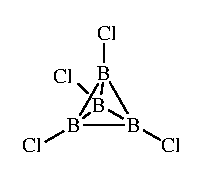
\includegraphics{picture/B4Cl4.eps}
        \end{minipage}
    }
    \subfigure[\ce{B8Cl8}的结构]{
        \begin{minipage}[b]{.3\linewidth}
            \centering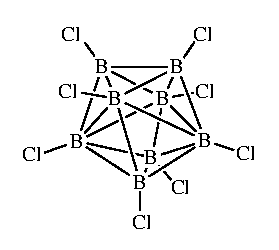
\includegraphics{picture/B8Cl8.eps}
        \end{minipage}
    }
    \subfigure[\ce{B9Cl9}的结构]{
        \begin{minipage}[b]{.3\linewidth}
            \centering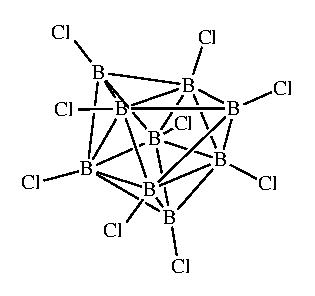
\includegraphics{picture/B9Cl9.eps}
        \end{minipage}
    }\caption{几种\ce{B_nCl_n}的结构}
\end{figure}
可以看到,它们的结构都和对应的\ce{[B_nH_n]^2-}相似,这是不符合Wade规则的又一例子.
\subsection{硼的含氧化合物}
硼(像硅一样)在自然界中总是以含氧化合物的形式存在,从来没有发现过单质硼或与其它非氧元素化合的硼\footnote{除了在意大利的Vesuvius火山口少量存在的氟硼钠石\ce{NaBF4}和氟硼钾铯石\ce{(K,Cs)BF4}.}.这些物质都具有复杂的结构,因此是一个值得探讨的内容.
\subsubsection{硼的氧化物}
\begin{substance}[\ce{B2O3}]
    三氧化二硼,化学式为\ce{B2O3},一般情况下为白色蜡状固体,但也可以形成为黑色玻璃态.\ce{B2O3}的熔点为$450\tc$,沸点为$1650\tc$.
\end{substance}
\ce{B2O3}是最难结晶的几种物质之一.它总是凝固形成玻璃态,而晶体$\alpha$-\ce{B2O3}则需要通过对无水\ce{H3BO3}小心加热脱水得到.无论何种形态,都以平面三角形的三配位\ce{\{BO3\}}单元为结构的基础,形成无限延伸的结构.
\begin{figure}[H]
    \subfigure[\ce{B2O3}的晶胞示意图]{
        \begin{minipage}[b]{.45\linewidth}
            \centering\includegraphics[scale=0.1]{picture/B2O3-1.eps}
        \end{minipage}
    }
    \subfigure[\ce{B2O3}的四倍晶胞示意图]{
        \begin{minipage}[b]{.45\linewidth}
            \centering\includegraphics[scale=0.1]{picture/B2O3-2.eps}
        \end{minipage}
    }\caption{\ce{B2O3}的晶体结构}
\end{figure}
气态的\ce{B2O3}以单体\ce{O=B-O-B=O}的形式存在.\\
\indent \ce{B2O3}作为酸性氧化物和各种金属氧化物都能在熔融时化合生成具有鲜艳颜色的偏硼酸盐,并且颜色随着金属元素不同而不同.这就是著名的硼砂珠实验(实际操作可以直接加热硼砂与金属氧化物的混合物).\\
\indent \ce{B2O3}主要用于制造含硼玻璃.高硼硅玻璃的热膨胀系数更低,因此在冷却时受到的温度梯度应力更小,因此相比普通玻璃有更强的抗断裂性能.\\
\indent 将\ce{B2Cl4}水解即可得到\ce{B2(OH)4},然后再加热脱水即可得到硼的低氧化物\ce{(BO)_n}.这一物质在硼化物的制备中已经提到过.将硼单质与\ce{B2O3}共热亦可得到这种物质:
\begin{center}
    \ce{B2O3 + B -> 3BO}
\end{center}
因此,在过量硼单质存在的反应中,应当考虑这种物质的生成.
\subsubsection{硼的含氧酸}
\paragraph{硼酸\ce{H3BO3}}
\ce{H3BO3}是大多数硼化合物水解的最终正常产物,通常可由酸化硼砂的水溶液得到.
\begin{substance}[\ce{H3BO3}]
    硼酸,又称原硼酸,化学式为\ce{H3BO3}(写作\ce{B(OH)3}也许更合适).硼酸是白色粉末或片状白色透明晶体,在$169\tc$发生脱水生成偏硼酸.
\end{substance}
硼酸晶体中有着无限延伸的层状结构,层内的\ce{H3BO3}分子通过氢键相互连接,而层间距离则较大.这也解释了硼酸晶体的分层裂解性能和较低的密度.
\chemfig{H3BO3}{1}{\ce{H3BO3}的层状结构}
\indent 硼酸是一元弱酸,其酸性是通过接受\ce{OH-}而非电离出\ce{H+}实现的:
\begin{center}
    \ce{H3BO3 + 2H2O <=> H3O+ + [B(OH)4]-}\ \ \ $\text pK_\text a=9.25$
\end{center}
向硼酸水溶液中加入多羟基醇可以显著增强其酸性.形成螯合物在熵效应上占明显优势,因而能使平衡明显右移.
\begin{center}
    \ce{H3BO3 + 2Me2C(OH)C(OH)Me2 -> [B(Me2COCOMe2)2]- + H3O+ + 2H2O}\\
    \ce{H3BO3 + 2HOCH2C(OH)CH2OH -> [B(OCH2C(OH)CH2O)2]- + H3O+ + 2H2O}
\end{center}
生成的螯合离子的结构如下所示.
\begin{figure}[H]
    \subfigure[\ce{[B(Me2COCOMe2)2]-}的结构示意图]{
        \begin{minipage}[b]{.45\linewidth}
            \centering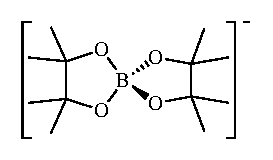
\includegraphics{picture/B(ORRO)2-1.eps}
        \end{minipage}
    }
    \subfigure[\ce{[B(OCH2C(OH)CH2O)2]-}的结构示意图]{
        \begin{minipage}[b]{.45\linewidth}
            \centering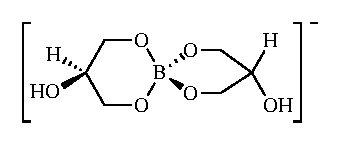
\includegraphics{picture/B(ORRO)2-2.eps}
        \end{minipage}
    }\caption{硼酸多羟基醇酯阴离子的结构}
\end{figure}
我们在介绍浓硫酸的性质时已经说过\ce{H3BO3}在硫酸中生成\ce{[B(HSO4)4]-},因而表现得像强酸:
\begin{center}
    \ce{H3BO3 + 6H2SO4 -> 3H3O+ + 2HSO4- + [B(HSO4)4]-}
\end{center}
硼酸与\ce{ROH/H2SO4}反应即可得到对应的硼酸酯\ce{B(OR)3}.它与\ce{H2O2}也可以反应得到过一硼酸盐\ce{[HOOB(OH)3]-}和过硼酸盐\ce{[B2(OH)4(O2)2]^2-},结构分别如下:
\begin{figure}[H]
    \subfigure[\ce{[HOOB(OH)3]-}的结构示意图]{
        \begin{minipage}[b]{.45\linewidth}
            \centering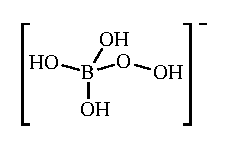
\includegraphics{picture/HOOB(OH)3-.eps}
        \end{minipage}
    }
    \subfigure[\ce{[B2(OH)4(O2)2]^2-}的结构示意图]{
        \begin{minipage}[b]{.45\linewidth}
            \centering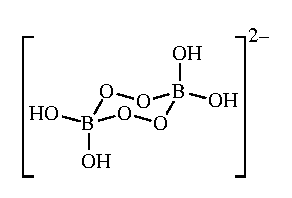
\includegraphics{picture/B2(OH)4(O2)22-.eps}
        \end{minipage}
    }\caption{过氧硼酸根的结构}
\end{figure}
\paragraph{偏硼酸\ce{HBO2}}
加热硼酸使其部分脱水即可得到偏硼酸\ce{HBO2}.正交\ce{HBO2}中存在其三聚体\ce{B3O3(OH)3},其层状结构如下:
\chemfig{HBO2}{1}{正交\ce{HBO2}的层状结构}
因此也可以看出,具有$C_3$轴的\ce{B3O3(OH)3}是更稳定的构象异构体.
\subsubsection{硼酸盐}
\paragraph{硼酸盐结构综述}
大体而言,硼酸盐中的\ce{B}总是平面三角形构型或四面体构型的.我们把一些典型硼酸盐的阴离子结构和对应的盐给出如下.
\begin{figure}[H]
    \centering
    \subfigure[\ce{[BO3]^3-} \ce{Mg3(BO3)2,LaBO3}]{
        \begin{minipage}[b]{.23\linewidth}
            \centering
\includegraphics{picture/BO33-.eps}
        \end{minipage}
    }
    \subfigure[\ce{[B2O5]^4-} \ce{Mg2B2O5,Fe2B2O5}]{
        \begin{minipage}[b]{.23\linewidth}
            \centering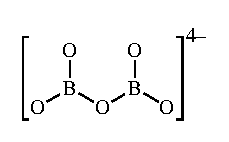
\includegraphics{picture/B2O54-.eps}
        \end{minipage}
    }
    \subfigure[\ce{[B3O6]^3-} \ce{K3B3O6,BaB2O4}]{
        \begin{minipage}[b]{.23\linewidth}
            \centering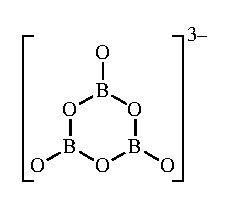
\includegraphics{picture/B3O63-.eps}
        \end{minipage}
    }
    \subfigure[\ce{[BO2]^{n-}_n} \ce{Ca(BO2)2}]{
        \begin{minipage}[b]{.23\linewidth}
            \centering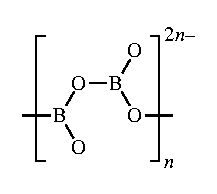
\includegraphics{picture/BO2-.eps}
        \end{minipage}
    }\caption{硼酸盐阴离子的结构I$-$平面三角形配位的硼酸根阴离子}
\end{figure}
\begin{figure}[H]
    \centering
    \subfigure[\ce{[BO4]^5-} \ce{TaBO4}]{
        \begin{minipage}[b]{.4\linewidth}
            \centering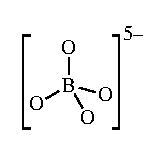
\includegraphics{picture/BO45-.eps}
        \end{minipage}
    }
    \subfigure[\ce{[B(OH)4]-} \ce{Na[B(OH)4]}]{
        \begin{minipage}[b]{.4\linewidth}
            \centering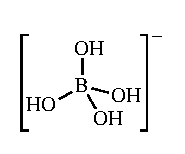
\includegraphics{picture/B(OH)4-.eps}
        \end{minipage}
    }
    \subfigure[\ce{[B2O(OH)6]^2-} \ce{Mg[B2O(OH)6]}]{
        \begin{minipage}[b]{.4\linewidth}
            \centering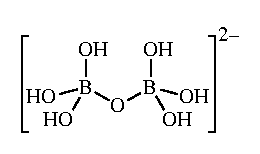
\includegraphics{picture/B2O(OH)62-.eps}
        \end{minipage}
    }
    \subfigure[\ce{[B2(OH)4(O2)2]^2-} \ce{NaBO3.4H2O}]{
        \begin{minipage}[b]{.4\linewidth}
            \centering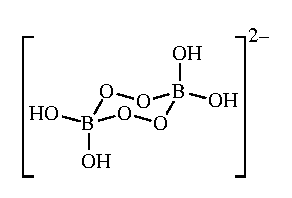
\includegraphics{picture/B2(OH)4(O2)22-.eps}
        \end{minipage}
    }\caption{硼酸盐阴离子的结构II$-$四面体配位的硼酸根阴离子}
\end{figure}
\begin{figure}[H]
    \centering
    \subfigure[\ce{[B5O6(OH)4]-} \ce{K[B5O6(OH)4].2H2O}]{
        \begin{minipage}[b]{.3\linewidth}
            \centering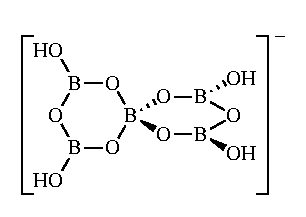
\includegraphics{picture/B5O6(OH)4-.eps}
        \end{minipage}
    }
    \subfigure[\ce{[B3O3(OH)5]^2-} \ce{Ca[B3O3(OH)5].H2O}]{
        \begin{minipage}[b]{.3\linewidth}
            \centering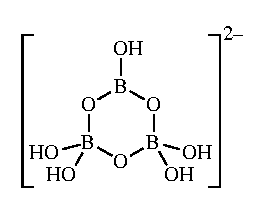
\includegraphics{picture/B3O3(OH)52-.eps}
        \end{minipage}
    }
    \subfigure[\ce{[B4O5(OH)4]^2-} \ce{Na2[B4O5(OH)4].8H2O}]{
        \begin{minipage}[b]{.3\linewidth}
            \centering\includegraphics{picture/B4O5(OH4)2--1.eps}
        \end{minipage}
    }\caption{硼酸盐阴离子的结构III$-$兼有三配位和四配位硼的硼酸根阴离子}
\end{figure}
\paragraph{硼砂}
作为一种使用历史悠久的矿物,有关硼砂有很多值得了解的内容.
\begin{substance}[\ce{Na2B4O7.10H2O}]
    硼砂(Borax),化学式为\ce{Na2B4O7.10H2O},为质地较软的白色粉末或无色晶体.硼砂略带甜味和咸味,易溶于水,置于空气中则容易失去结晶水而风化.硼砂有一定毒性,摄入可能导致肝肾功能受损和内分泌紊乱.
\end{substance}
\subparagraph{硼砂的历史}
中国是最早发现和使用硼砂的国家之一.这种盛产于西藏,青海\footnote{据说有人在某年初赛时看到青海湖就推出了硼砂.}等地的矿物最初被用作金属助焊剂,因而硼砂最初被称作\tbf{焊剂}(tincal).在公元8世纪,源自西藏,波斯和亚洲其它地区的天然硼砂通过丝绸之路被运往西方.硼砂的英文名Borax则可能来源于波斯语Burah,意为“白色闪亮的矿物”.
\subparagraph{硼砂的结构}
虽然硼砂经常地被写作\ce{Na2B4O7.10H2O},但事实上其中的阴离子为\ce{[B4O5(OH)4]^2-}.晶体中的离子通过氢键连接形成长链.\ce{Na+}被\ce{H2O}六配位而形成八面体,八面体共边连接形成另一种长链.两种长链通过氢键连接,作用力相对较弱,因而硼砂晶体质地较软.
\begin{figure}[H]
    \centering
    \subfigure[\ce{[B4O5(OH4)]^2-}离子的立体结构示意图]{
        \begin{minipage}[b]{.33\linewidth}
            \centering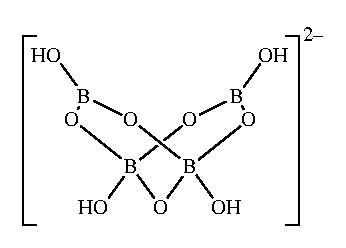
\includegraphics{picture/B4O5(OH4)2--2.eps}
        \end{minipage}
    }
    \subfigure[硼砂中\ce{[B4O5(OH4)]^2-}形成的长链]{
        \begin{minipage}[b]{.63\linewidth}
            \centering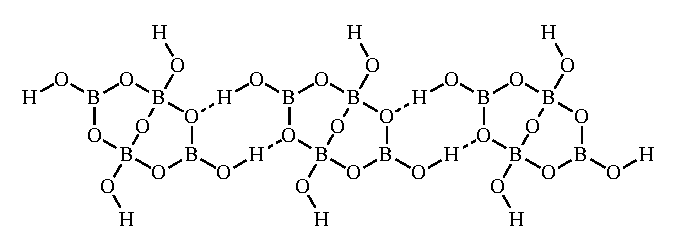
\includegraphics{picture/B4O5(OH4)2--3.eps}
        \end{minipage}
    }\caption{硼砂的相关结构}
\end{figure}
\subparagraph{硼砂的化学性质}
硼砂容易失水.加热到$75\tc$,即失水得到\ce{NaB4O7.5H2O},再加热到$200\tc$即得到\ce{Na2B4O7},即无水硼砂.无水硼砂中并没有分立的\ce{[B4O7]^2-},而是形成复杂的网状结构.\\
\indent 硼砂水溶液是天然的缓冲溶液.这是因为\ce{[B4O5(OH)4]^2-}水解的方式如下:
\begin{center}
    \ce{[B4O5(OH)4]^2- + 5H2O -> 2[B(OH)4]- + 2B(OH)3}
\end{center}
恰好产生比例为$1:1$的硼酸和硼酸阴离子,形成缓冲对.
\paragraph{含\ce{B-O}键的有机化合物}
硼酸酯大多含有三配位的硼.\\
\indent 最简单的三硼酸酯\ce{B(OMe)3}可以由\ce{B2O3}或\ce{H3BO3}与\ce{MeOH}反应得到.它燃烧时产生的特征绿色火焰是鉴定\ce{B}元素的一种手段.\\
\indent 对\ce{H3BO3}的不完全烷基化可以得到\ce{RB(OH)2}.它可以脱水三聚形成含有\ce{B-O}六元环的\ce{B3O3R3},其结构与\ce{HBO2}的三聚体相似.
\subsection{硼氮化合物}
\paragraph{氮化硼\ce{BN}}
氮化硼的概述如下.
\begin{substance}[\ce{BN}]
    氮化硼,化学式为\ce{BN}.六方$\alpha$-\ce{BN}又称白石墨,是白色固体.立方$\beta$-\ce{BN}是类似金刚石的固体,为无色到琥珀色的极坚硬的固体.
\end{substance}
\subparagraph{\ce{BN}的制备}
制备\ce{BN}有很多技术困难.实验室通常采用熔融硼砂和氯化铵的混合物:
\begin{center}
    \ce{Na2B4O7.10H2O + 4NH4Cl ->T[熔融] 2NaCl + 2HCl + 17H2O + 4BN}
\end{center}
工业上大规模的合成可以采取硼酸与尿素在\ce{NH3}气氛中共热得到:
\begin{center}
    \ce{2H3BO3 + 6CO(NH2)2 ->T[熔融][\ce{NH3}] 2BN + 6CO2 + 10NH3}
\end{center}
“只有勇敢的或十足傻瓜的化学家才企图写出这两个反应的配平的方程式.”\footnote{N. N. Greenwood, A. Earnshaw. 元素化学[M]. 北京:高等教育出版社, 1997.}尽管Greenwood如此写道,但笔者认为配平这两个方程式仍是应当掌握的知识.另外一种方式是将\ce{NH3}与\ce{BF3}反应的产物\ce{H3NBF3}加热:
\begin{center}
    \ce{4H3NBF3 ->T[$\Delta$] 3NH4BF4 + BN}
\end{center}
\subparagraph{\ce{BN}的结构}
六方$\alpha$-\ce{BN}的结构与石墨大体上比较相似,是由\ce{B-N}六元环构成的平面结构堆叠而成.然而不同的是,石墨中的各层是交错重叠的(这也衍生出了三方石墨和六方石墨两种晶型),而六方$\alpha$-\ce{BN}的两层是完全重叠的,每个\ce{B}原子与上下两层的\ce{N}原子在投影上对齐.这可能是静电相互作用导致的.此外,其中的\ce{B-N}键键长为$135\text{ pm}$,明显短于正常的\ce{B-N}键,因此说明其有明显的$\pi$键性质.
\chemfig{alpha-BN}{0.1}{六方$\alpha$-\ce{BN}的晶胞}
六方$\alpha$-\ce{BN}因其层状结构和较弱的层间作用力而可以作为优良的润滑剂.\\
\indent 在高温高压下,六方$\alpha$-\ce{BN}可以转化为闪锌矿型的立方$\beta$-\ce{BN}或纤锌矿型的六方$\beta$-\ce{BN}.
\subparagraph{\ce{BN}的性质与反应}
尽管六方$\alpha$-\ce{BN}键长平均化,但它并不像石墨一样非常稳定.在氟化氢的作用下,\ce{BN}可以转化为\ce{NH4BF4},而氟气则定量地使其转化为\ce{N2}和\ce{BF3}:
\begin{center}
    \ce{BN + 4HF -> NH4BF4}\\
    \ce{2BN + 3F2 -> 2BF3 + N2}
\end{center}

\end{document}